%% Manuscript for submission to Computers in Biology and Medicine (Elsevier).
%% Build: latexmk -pdf manuscript.tex   (or ./build.sh, which also builds figures, highlights and cover letter)
\documentclass[preprint,12pt,authoryear=false]{elsarticle}

\usepackage[T1]{fontenc}
\usepackage{lmodern}
\usepackage{amsmath,amssymb}
\usepackage{graphicx}
\usepackage{booktabs}
\usepackage{tabularx}
\usepackage{array}
\usepackage{multirow}
\usepackage{xcolor}
\usepackage{lineno}
\usepackage{xurl}
\usepackage[hidelinks]{hyperref}
\usepackage{siunitx}
\usepackage[font=small,labelfont=bf]{caption}
\usepackage{rotating}
\usepackage[section]{placeins}

\graphicspath{{figures/}}
\newcolumntype{L}{>{\raggedright\arraybackslash}X}
\biboptions{sort&compress}
\modulolinenumbers[5]
\linenumbers

\journal{Computers in Biology and Medicine}

% Drop the title-page "Preprint submitted to" footer, which collides with the author footnote.
\makeatletter
\def\ps@pprintTitle{\let\@oddhead\@empty\let\@evenhead\@empty\let\@oddfoot\@empty\let\@evenfoot\@empty}
\makeatother

\begin{document}

\begin{frontmatter}

\title{Leakage-controlled stacking and recursive feature elimination for type~2 diabetes prediction: a rigorous evaluation on the PIMA dataset}

%% TODO(author): confirm name, affiliation and ORCID before submission.
\author[anits]{Subrahmanyam Tanala\corref{cor1}}
\ead{subrahmanyam.eee@anits.edu.in}
\cortext[cor1]{Corresponding author.}
\affiliation[anits]{organization={Department of Electrical and Electronics Engineering, Anil Neerukonda Institute of Technology and Sciences (ANITS)},
            city={Visakhapatnam},
            state={Andhra Pradesh},
            country={India}}

\begin{abstract}
\noindent\textbf{Background:} Machine-learning models for type~2 diabetes mellitus (T2DM) screening often report optimistic performance because imputation or feature selection is fitted before validation, and because differences between models are rarely tested statistically.

\noindent\textbf{Methods:} We built a leakage-controlled pipeline that combines median imputation of impossible zero values, eight engineered clinical features, recursive feature elimination with cross-validation (RFECV) and an eight-learner stacking ensemble with a logistic-regression meta-learner. Every step was re-fitted inside each validation split. On the PIMA Indians Diabetes dataset (768 women, 268 with diabetes), we compared 11 learners with and without a common RFECV subset using 5$\times$10-fold repeated cross-validation with corrected confidence intervals and Holm-adjusted tests. Results were confirmed on a 154-patient hold-out set with bootstrap intervals and DeLong tests. We also assessed calibration, sensitivity-targeted thresholds, decision curves, alternative imputation strategies and SHAP explanations.

\noindent\textbf{Results:} RFECV reduced the inputs by 25\% without loss of discrimination; glucose, BMI, family history and their interactions were consistently retained. Cross-validated ROC-AUC was 0.843 (95\% CI 0.809--0.878) for RFECV + stacking and 0.842 (0.809--0.875) for logistic regression (adjusted $p = 1.00$). On the hold-out set, RFECV + stacking achieved sensitivity 0.815, specificity 0.740, MCC 0.532 and ROC-AUC 0.822. These were the highest observed sensitivity and MCC, but no ROC-AUC difference was significant. Class weighting caused systematic risk overestimation (calibration intercept $-0.62$, slope 1.00).

\noindent\textbf{Conclusions:} Under rigorous, leakage-free validation, stacking and RFECV give compact, sensitivity-oriented models but no discrimination gain over logistic regression on this small cohort. Calibration and threshold choice deserve as much attention as model choice.
\end{abstract}


\begin{keyword}
Type 2 diabetes mellitus \sep Stacked generalisation \sep Recursive feature elimination \sep Data leakage \sep Calibration \sep Decision curve analysis \sep PIMA Indians Diabetes
\end{keyword}

\end{frontmatter}

\section{Introduction}
\label{sec:intro}

An estimated 536.6 million adults aged 20--79 years were living with diabetes in 2021, and this number is projected to reach 783.2 million by 2045~\cite{sun2022idf}. Type~2 diabetes mellitus (T2DM) accounts for the large majority of cases, and a substantial share of people with diabetes are undiagnosed~\cite{idf2021}. Because hyperglycaemia damages the kidneys, retina, nerves and vasculature years before symptoms appear, risk estimates from routinely collected measurements could help prioritise confirmatory testing and follow-up.

Machine-learning (ML) classifiers trained on variables such as plasma glucose, body-mass index (BMI), blood pressure and familial risk are a common route to such risk-prediction tools. Two design decisions dominate this literature. The first is feature selection: wrapper methods such as recursive feature elimination (RFE)~\cite{guyon2002rfe,kohavi1997wrappers} prune redundant inputs, and RFE with cross-validation (RFECV) chooses the subset size by validated performance. The second is model choice: stacked generalisation~\cite{wolpert1992stacked} trains a meta-learner on the out-of-fold predictions of diverse base learners and is often reported to outperform any single learner.

On small clinical datasets, however, the reported gains of such pipelines are hard to interpret. Imputation, scaling, oversampling or feature selection are frequently fitted on the complete dataset before cross-validation or splitting. This leaks information from the evaluation data into model development and inflates performance~\cite{ambroise2002selection,kaufman2012leakage,kapoor2023leakage}. Moreover, differences between models are usually reported without confidence intervals or paired tests, calibration is rarely assessed~\cite{vancalster2019calibration}, and the default 0.5 decision threshold is seldom justified for the intended use. Systematic comparisons have also found no average performance benefit of flexible ML over logistic regression for clinical prediction~\cite{christodoulou2019}.

This study therefore asks a deliberately narrow question: \emph{when every data-dependent step is kept inside the validation loop, does combining RFECV with a heterogeneous stacking ensemble improve T2DM prediction on the PIMA cohort over simpler models, and how do calibration and the choice of operating threshold affect its interpretation?} The contribution is a rigorous evaluation framework, not a new learning algorithm:

\begin{enumerate}
  \item A leakage-controlled pipeline in which median imputation of physiologically impossible zeros, clinically motivated feature engineering, standardisation, RFECV and an eight-learner stacking ensemble are all re-fitted within the training part of every split.
  \item A common feature-selection protocol in which RFECV is fitted once per outer fold and its subset is shared by every compared learner, together with a learner-specific RFECV sensitivity analysis for logistic regression.
  \item A statistically explicit evaluation: 5$\times$10-fold repeated cross-validation with corrected confidence intervals and corrected resampled $t$-tests~\cite{nadeau2003inference,bouckaert2004replicability}, Holm adjustment for multiplicity~\cite{holm1979}, bootstrap confidence intervals and DeLong tests~\cite{delong1988,sun2014delong} on an untouched hold-out set.
  \item A clinically oriented assessment that goes beyond discrimination: calibration, pre-specified sensitivity-targeted thresholds, decision-curve analysis~\cite{vickers2006dca}, a missing-data sensitivity analysis and SHAP explanations~\cite{lundberg2017shap}.
\end{enumerate}

We report where the framework helps and where it does not. In particular, under strict validation and prespecified hyperparameters, the stacking ensemble does not discriminate better than regularised logistic regression on this cohort. Because PIMA predictors include 2-h oral glucose tolerance test (OGTT) values, the setting is risk stratification among people who have already had an OGTT, not population-level screening, and the analysis is primarily a methodological benchmark.

\section{Related work}
\label{sec:related}

\paragraph{Machine learning on the PIMA cohort}
The PIMA Indians Diabetes dataset originates from a long-running longitudinal study of the Gila River Indian Community~\cite{knowler1978} and was introduced as an ML benchmark with the ADAP neural network~\cite{smith1988adap}. It has since been used to evaluate logistic regression, support vector machines, tree ensembles such as random forests~\cite{breiman2001rf}, XGBoost~\cite{chen2016xgboost} and LightGBM~\cite{ke2017lightgbm}, and deep networks. Reported accuracies range from about 0.75 to above 0.98. Recent examples include a Boruta and stacking model reporting 98\% accuracy~\cite{zhou2023boruta} and an RFE--GRU network reporting 90.7\% accuracy~\cite{shams2025rfegru}. By contrast, Reza et al.\ reported 75.0\% (train--test split) and 77.1\% (cross-validation) for a stacked model on PIMA~\cite{reza2024stacking}. A spread this wide on a fixed 768-patient dataset is more plausibly explained by differences in validation design than by differences between algorithms.

\paragraph{Stacking and feature selection for diabetes}
Wolpert introduced stacked generalisation~\cite{wolpert1992stacked}, and Ting and Witten showed that stacking works best when a simple linear meta-learner receives class probabilities~\cite{ting1999issues}. In this journal, Kalagotla et al.\ combined correlation-based feature selection with a stack of a multilayer perceptron, SVM and logistic regression on PIMA~\cite{kalagotla2021stacking}. Idris et al.\ combined stacking with RFE and isolation-forest outlier removal and reported 79.1\% accuracy on PIMA~\cite{idris2024stacking}. The combination of RFE-type selection and stacking is therefore not new. What is less common is (i) validating the \emph{whole} chain, including imputation and selection, without leakage; (ii) quantifying uncertainty and testing differences between models; and (iii) reporting calibration and clinical utility alongside discrimination.

\paragraph{Leakage, selection bias and reporting}
Ambroise and McLachlan showed that selecting features on the full dataset before cross-validation gives strongly optimistic error estimates~\cite{ambroise2002selection}. Varma and Simon showed a similar bias when tuning and evaluation share folds~\cite{varma2006bias}. Kaufman et al.\ formalised data leakage~\cite{kaufman2012leakage}, and Kapoor and Narayanan documented leakage across hundreds of ML-based studies in 17 fields~\cite{kapoor2023leakage}. The TRIPOD+AI statement now asks prediction-model studies to report how missing data were handled, how performance was validated, and how calibration and clinical utility were assessed~\cite{collins2024tripodai}. Our evaluation design follows these recommendations.

\section{Materials and methods}
\label{sec:methods}

Fig.~\ref{fig:pipeline} summarises the framework. This study is reported following the TRIPOD+AI recommendations where applicable~\cite{collins2024tripodai}.

\begin{figure*}[!htbp]
  \centering
  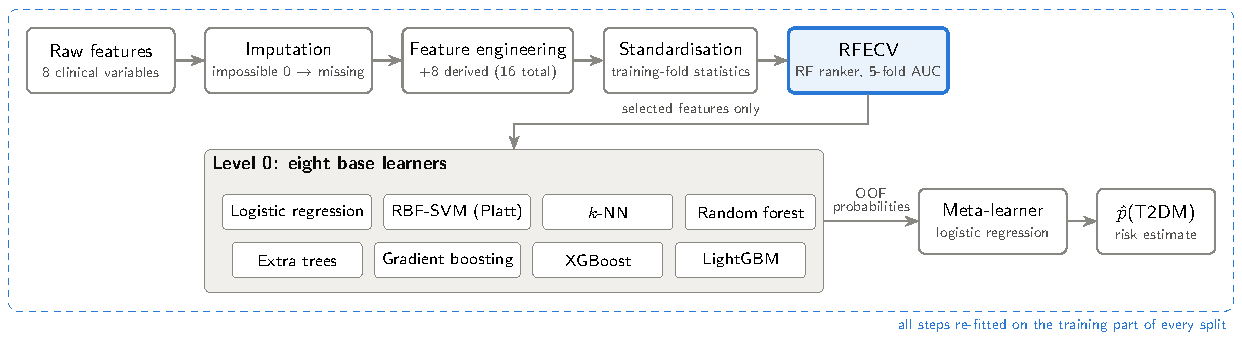
\includegraphics[width=\textwidth]{fig1_pipeline.pdf}
  \caption{Proposed pipeline. Imputation, feature engineering, standardisation and RFECV are fitted on the training part of each split only. The features retained by RFECV are passed to eight heterogeneous base learners, whose out-of-fold (OOF) probabilities train a logistic-regression meta-learner.}
  \label{fig:pipeline}
\end{figure*}

\subsection{Data}
We used the PIMA Indians Diabetes dataset~\cite{smith1988adap}: 768 women of Pima heritage aged at least 21 years, of whom 268 (34.9\%) had diabetes. Each record contains eight predictors: number of pregnancies, 2-h plasma glucose concentration in an oral glucose tolerance test (OGTT; mg/dL), diastolic blood pressure (mm\,Hg), triceps skin-fold thickness (mm), 2-h serum insulin (\textmu U/mL), BMI (kg/m$^2$), diabetes pedigree function and age (years). The data are publicly available and de-identified~\cite{pimadata}.

\paragraph{Outcome definition and intended setting} According to the dataset documentation, the binary outcome indicates whether the woman showed signs of diabetes according to World Health Organization criteria, i.e.\ a 2-h post-load plasma glucose of at least 200~mg/dL at a survey examination or diagnosis during routine medical care~\cite{pimadata,smith1988adap}. This outcome is not a contemporary clinical diagnosis of T2DM based on current HbA1c or fasting-glucose criteria~\cite{ada2024}. Moreover, the strongest predictor, 2-h OGTT glucose, is itself a diagnostic measurement closely related to the outcome definition. The models studied here therefore address risk stratification among individuals for whom OGTT measurements are already available, not low-cost population screening. We treat the analysis primarily as a methodological benchmark rather than as the development of a clinically deployable diagnostic model.

\subsection{Missing values}
Zero is physiologically impossible for glucose, blood pressure, skin-fold thickness, insulin and BMI, so these zeros were recoded as missing (Table~\ref{tab:missing-counts}). In the primary analysis, missing values were replaced by the median of the training data in each split. Because insulin is missing for almost half of the patients, we also compared three alternatives in a sensitivity analysis (Section~\ref{sec:missing-methods}).

\begin{table}[!htbp]
\centering
\caption{Physiologically impossible zero values recoded as missing ($n = 768$).}
\label{tab:missing-counts}
\begin{tabular}{lrr}
\toprule
Predictor & Missing ($n$) & Missing (\%) \\
\midrule
Insulin & 374 & 48.7 \\
Skin-fold thickness & 227 & 29.6 \\
Diastolic blood pressure & 35 & 4.6 \\
BMI & 11 & 1.4 \\
Glucose & 5 & 0.7 \\
\bottomrule
\end{tabular}
\end{table}

\subsection{Feature engineering}
Eight derived features encoding known T2DM risk interactions were added after imputation, giving 16 candidate predictors for RFECV: the 8 original variables and 8 deterministic derived features (Table~\ref{tab:features}). Because the derived features are functions of the original variables, the 16 candidates are not informationally independent. The insulin-resistance term follows the HOMA-IR formula~\cite{matthews1985homa}, but PIMA records 2-h post-load rather than fasting glucose and insulin. We therefore name it \texttt{HOMA\_IR\_surrogate} and do not interpret it as clinical HOMA-IR. The binary thresholds follow the WHO obesity cut-off~\cite{who2000obesity} and the 2-h OGTT threshold for impaired glucose tolerance~\cite{ada2024}.

\begin{table}[!htbp]
\centering
\caption{Derived features. All continuous inputs are measured after imputation.}
\label{tab:features}
\small
\begin{tabularx}{\linewidth}{llL}
\toprule
Feature & Definition & Rationale \\
\midrule
\texttt{Glucose\_BMI} & Glucose $\times$ BMI / 100 & Joint glycaemia--adiposity effect \\
\texttt{Glucose\_Age} & Glucose $\times$ Age / 100 & Glycaemic risk rising with age \\
\texttt{HOMA\_IR\_surrogate} & Glucose $\times$ Insulin / 405 & Insulin-resistance surrogate (post-load) \\
\texttt{Insulin\_Glucose\_Ratio} & Insulin / Glucose & Insulin response relative to glucose \\
\texttt{BMI\_Age} & BMI $\times$ Age / 100 & Cumulative adiposity exposure \\
\texttt{Obese} & $1$ if BMI $\geq 30$ & WHO obesity threshold \\
\texttt{IGT\_2h} & $1$ if Glucose $\geq 140$ & Impaired glucose tolerance threshold \\
\texttt{Pedigree\_Age} & Pedigree $\times$ Age & Familial risk expressed over time \\
\bottomrule
\end{tabularx}
\end{table}

\subsection{Recursive feature elimination with cross-validation}
All features were standardised with training statistics. RFECV started from the 16 candidate predictors. At each step it fitted a random forest (200 trees, balanced class weights), ranked features by impurity-based importance and removed the least important one. Each subset size was scored by stratified 5-fold cross-validated ROC-AUC within the training data, and the size with the highest mean score was retained (minimum three features).

\paragraph{Common versus learner-specific selection}
In the model comparison, RFECV was fitted once within each outer training fold using the random-forest ranking estimator, and the resulting subset was supplied to every candidate learner. This gives all learners an identical, leakage-free feature-selection protocol at the cost of one RFECV fit per fold. The subset is optimised with the random-forest ranking criterion, not separately for each learner. It is therefore \emph{not} equivalent to cross-validating a learner-specific RFECV pipeline for every classifier. To gauge the effect of this choice, we also evaluated logistic regression with its own RFECV ranked by absolute standardised coefficients (``LR-ranked RFECV''). Throughout the article, ``+ RFECV'' denotes the common random-forest-ranked RFECV subset.

\subsection{Stacking ensemble}
The level-0 learners were chosen for diversity of inductive bias (Table~\ref{tab:learners}). The level-1 meta-learner was an L2-regularised logistic regression with balanced class weights. It was trained on the positive-class probabilities produced by each base learner for held-out samples in an internal stratified 5-fold split~\cite{wolpert1992stacked,ting1999issues}. The base learners were then refitted on all training data for prediction. Gaussian naive Bayes and a depth-5 decision tree were evaluated as additional reference learners but were not part of the stack. Hyperparameters were fixed a priori at conventional settings for small tabular data (Table~\ref{tab:learners}): library defaults where these are standard (e.g.\ $C=1$ for LR and SVM), moderate ensemble sizes (200--300 trees), shallow boosting (depth 3) with a small learning rate (0.05), and a neighbourhood of $k=15$. They were not tuned, so that no tuning loop could leak into the evaluation. All comparisons between learners are therefore conditional on these prespecified configurations and do not cover every possible tuned version of each algorithm.

\begin{table}[!htbp]
\centering
\caption{Level-0 learners and their fixed settings.}
\label{tab:learners}
\small
\begin{tabularx}{\linewidth}{llL}
\toprule
Learner & Family & Settings \\
\midrule
Logistic regression (LR) & Linear & L2, $C=1$, balanced class weights \\
SVM & Kernel & RBF, $C=1$, balanced weights, Platt-calibrated~\cite{platt1999} \\
$k$-nearest neighbours & Instance-based & $k=15$, distance-weighted \\
Random forest~\cite{breiman2001rf} & Bagged trees & 300 trees, min.\ leaf 2, balanced weights \\
Extra trees & Randomised trees & 300 trees, min.\ leaf 2, balanced weights \\
Gradient boosting & Boosted trees & 200 trees, depth 3, learning rate 0.05 \\
XGBoost~\cite{chen2016xgboost} & Boosted trees & 300 trees, depth 3, rate 0.05, subsample 0.8 \\
LightGBM~\cite{ke2017lightgbm} & Boosted trees & 300 trees, 15 leaves, rate 0.05, balanced weights \\
\bottomrule
\end{tabularx}
\end{table}

\subsection{Internal evaluation design}
Supplementary Fig.~S1 shows where each loop runs. The data were split once into a stratified 80\% development set (614 patients, 214 with diabetes) and a 20\% hold-out set (154 patients, 54 with diabetes), with random seed 42. The split was fixed in code before any model was fitted. Hold-out results of the same prespecified pipeline were inspected in an earlier draft of this work; no learner, hyperparameter, feature or preprocessing choice was changed afterwards, and the hold-out set was not used for any modelling decision.

\paragraph{Repeated cross-validation}
On the development set, 11 learners (the eight base learners, naive Bayes, the decision tree and the stack) were compared with and without the common RFECV subset (22 configurations), together with logistic regression with LR-ranked RFECV (23 configurations in total; Supplementary Table~S5), using stratified 10-fold cross-validation repeated five times (50 folds). Within each fold, imputation, feature engineering, standardisation and RFECV were fitted on the nine training folds only. Because fold estimates from overlapping training sets are correlated, we report the mean of each metric with a 95\% confidence interval based on the Nadeau--Bengio corrected variance~\cite{nadeau2003inference},
\begin{equation}
  \widehat{\operatorname{Var}}_{\mathrm{corr}} = \left(\frac{1}{J} + \frac{n_{\mathrm{test}}}{n_{\mathrm{train}}}\right) s^2,
  \label{eq:corrected}
\end{equation}
where $J=50$ is the number of fold estimates, $s^2$ their sample variance, and $n_{\mathrm{test}}/n_{\mathrm{train}} = 1/9$. Each configuration was compared with logistic regression on all features using the corrected resampled $t$-test on paired fold differences ($J-1$ degrees of freedom)~\cite{nadeau2003inference,bouckaert2004replicability}. $p$-values were adjusted for the 22 comparisons with the Holm procedure~\cite{holm1979}. The comparison set was fixed in the analysis code before the repeated cross-validation was run. We chose this test because it is the standard, simulation-validated correction for the dependence between repeated cross-validation folds and has acceptable type~I error and good replicability~\cite{nadeau2003inference,bouckaert2004replicability}. A nested or paired bootstrap of the whole pipeline would have required refitting RFECV and the stack thousands of times (about 45~s per fit). The full testing procedure is given in Supplementary Section~S2.

\paragraph{Hold-out evaluation}
The final pipelines were fitted on the full development set and scored once on the hold-out set. ROC-AUC confidence intervals were computed with DeLong's method, and ROC-AUCs of correlated models were compared with DeLong's test~\cite{delong1988,sun2014delong}, with Holm adjustment over the six comparisons. All other metrics were given 95\% percentile bootstrap confidence intervals (2000 resamples of the hold-out patients).

\subsection{Performance measures}
We report accuracy, balanced accuracy, precision (positive predictive value, PPV), recall (sensitivity), specificity, F1, the Matthews correlation coefficient (MCC)~\cite{chicco2020mcc}, ROC-AUC and average precision. Calibration was assessed with the Brier score, calibration-in-the-large (the intercept $a$ of a logistic model with $\operatorname{logit}\hat p$ as offset), the calibration slope $b$ from $\operatorname{logit} P(y=1) = a' + b\,\operatorname{logit}\hat p$, and calibration curves~\cite{vancalster2019calibration}. A well-calibrated model has $a = 0$ and $b = 1$. Calibration was evaluated both on the pooled out-of-fold predictions of the development set and on the hold-out set. The pooled set contains 3070 predictions: each of the 614 unique development patients is predicted once in each of the five repeats. No recalibration was applied to the reported models. For reference, the development-set prevalence is $\pi = 214/614 = 0.349$, so an intercept correction for balanced class weighting would be $\operatorname{logit}(\pi) = -0.626$.

\subsection{Threshold and decision-curve analysis}
Instead of using the default 0.5 threshold, we pre-specified operating thresholds targeting 80\%, 85\%, 90\% and 95\% sensitivity. Each threshold was chosen on the development-set out-of-fold predictions, using one probability per patient (the mean over the five repeats). The threshold for a target sensitivity $s$ is the $\lceil s\,n_+\rceil$-th largest predicted probability among the $n_+ = 214$ development positives. Patients are flagged when their probability is greater than or equal to the threshold, so ties at the threshold are flagged and the development sensitivity is at least the target. The thresholds were then applied unchanged to the hold-out set, where sensitivity, specificity, PPV, NPV and the proportion of patients flagged were estimated with bootstrap confidence intervals. Potential clinical utility was assessed by internal decision-curve analysis~\cite{vickers2006dca} on the hold-out set, using the net benefit
\begin{equation}
  \mathrm{NB}(p_t) = \frac{\mathrm{TP}(p_t)}{n} - \frac{\mathrm{FP}(p_t)}{n}\cdot\frac{p_t}{1-p_t},
\end{equation}
over threshold probabilities $p_t$ from 0.05 to 0.60, and compared with treating all or no patients.

\subsection{Missing-data sensitivity analysis}
\label{sec:missing-methods}
We repeated the development-set comparison of logistic regression and stacking + RFECV (10-fold cross-validation repeated twice) with four imputation strategies, each fitted within the training folds: (i) median imputation; (ii) median imputation plus a binary missingness indicator for every predictor with missing values, which lets the model use informative missingness~\cite{sperrin2020missing}; (iii) iterative chained-equation imputation (scikit-learn \texttt{IterativeImputer}, Bayesian ridge, 20 iterations)~\cite{vanbuuren2011mice}; and (iv) $k$-nearest-neighbour imputation ($k=10$)~\cite{troyanskaya2001knn}. Differences from median imputation were tested with the corrected resampled $t$-test.

\subsection{Explainability}
We computed Shapley values~\cite{lundberg2017shap} for the hold-out predictions of the final stacking + RFECV pipeline. The pipeline was treated as one function of the eight raw clinical inputs. Because there are only eight inputs, the values were obtained by exact enumeration of all $2^8 = 256$ feature coalitions (SHAP \texttt{ExactExplainer}), with features outside a coalition replaced by values from 40 development-set patients drawn by simple random sampling with seed 42 (an interventional background). They are therefore exact with respect to this background distribution. SHAP values describe how much each input contributed to the model's predictions; they are attributions, not estimates of causal effects. Explanations are therefore expressed in clinically measured variables, not in engineered or standardised features.

\subsection{Implementation and reproducibility}
The framework was implemented in Python 3.11 with scikit-learn 1.9~\cite{pedregosa2011sklearn}, XGBoost 3.2, LightGBM 4.7 and SHAP. Every stochastic step used seed 42: the hold-out split, the repeated outer folds, the inner RFECV and stacking folds, all learners and the RFECV ranker, the iterative imputer, the bootstrap resampling and the SHAP background sample (Supplementary Section~S8). Code, configuration, the fold-level results and the scripts that generate every table and figure are publicly available (see Data availability). Every number reported here was produced from repository commit \texttt{e23102d}.

\section{Results}
\label{sec:results}

\subsection{Repeated cross-validation}
Table~\ref{tab:cv} and Fig.~\ref{fig:cv} summarise the 5$\times$10-fold comparison on the development set; Supplementary Table~S1 lists all nine metrics with confidence intervals for all 23 configurations. All learners except LightGBM and the single decision tree reached a mean ROC-AUC between 0.820 and 0.846, with overlapping corrected 95\% confidence intervals. Stacking on all 16 features had the highest mean ROC-AUC (0.846, 95\% CI 0.812--0.880), followed by stacking with the common RFECV subset (0.843, 0.809--0.878) and logistic regression on all features (0.842, 0.809--0.875). The differences between the stacks and logistic regression were small and not statistically significant (+0.004 and +0.001; Holm-adjusted $p = 1.000$ for both). After Holm adjustment, only LightGBM (0.803 and 0.800 without and with RFECV; adjusted $p = 0.044$ and $0.020$) and the decision tree (0.770 and 0.772; $p = 0.025$ and $0.020$) discriminated significantly worse than logistic regression. No configuration differed significantly from logistic regression in MCC.

At the default 0.5 threshold, the stacks had the highest mean sensitivity among the strong learners (0.763 without and 0.753 with RFECV, compared with 0.744 for logistic regression and 0.655 for the SVM), at the cost of lower specificity (0.757 compared with 0.775 and 0.840). The Platt-calibrated SVM had the lowest mean Brier score (0.156; stacking + RFECV 0.165).

The common RFECV subset changed mean ROC-AUC by at most 0.003 for every learner while reducing the inputs from 16 to a mean of 12.0 features (25\% fewer). Logistic regression with its own coefficient-ranked RFECV kept 10.1 features on average and reached a ROC-AUC of 0.840 (0.808--0.873). It performed no better than logistic regression with the common, random-forest-ranked subset (0.842) or with all features.

\begin{table*}[!htbp]
\centering
\caption{Development-set performance from 5$\times$10-fold repeated cross-validation (50 folds; $n = 614$). Values are means; Nadeau--Bengio corrected 95\% confidence intervals are shown in grey beneath. $\Delta$AUC is the mean paired difference from logistic regression on all features, with Holm-adjusted corrected resampled $t$-test $p$-values in brackets. ``+ RFECV'' denotes the common, random-forest-ranked RFECV subset. Sensitivity and specificity use a 0.5 threshold.}
\label{tab:cv}
\footnotesize
\setlength{\tabcolsep}{4pt}
\resizebox{\textwidth}{!}{%
\begin{tabular}{lrcccccl}
\toprule
Model & Features & ROC-AUC & MCC & Sens. & Spec. & Brier & $\Delta$AUC (adj.\ $p$) \\
\midrule
Stacking & 16.0 & 0.846 & 0.505 & 0.763 & 0.757 & 0.164 & +0.004 (1.000) \\
 &  & {\scriptsize\color{gray}(0.812--0.880)} & {\scriptsize\color{gray}(0.431--0.580)} &  &  &  &  \\[2pt]
Stacking + RFECV & 12.0 & 0.843 & 0.497 & 0.753 & 0.757 & 0.165 & +0.001 (1.000) \\
 &  & {\scriptsize\color{gray}(0.809--0.878)} & {\scriptsize\color{gray}(0.418--0.575)} &  &  &  &  \\[2pt]
Logistic regression & 16.0 & 0.842 & 0.507 & 0.744 & 0.775 & 0.163 & reference \\
 &  & {\scriptsize\color{gray}(0.809--0.875)} & {\scriptsize\color{gray}(0.438--0.576)} &  &  &  &  \\[2pt]
Logistic regression + RFECV & 12.0 & 0.842 & 0.492 & 0.717 & 0.782 & 0.163 & -0.000 (1.000) \\
 &  & {\scriptsize\color{gray}(0.811--0.873)} & {\scriptsize\color{gray}(0.418--0.566)} &  &  &  &  \\[2pt]
LR (LR-ranked RFECV) & 10.1 & 0.840 & 0.496 & 0.731 & 0.776 & 0.164 & -0.002 (1.000) \\
 &  & {\scriptsize\color{gray}(0.808--0.873)} & {\scriptsize\color{gray}(0.426--0.567)} &  &  &  &  \\[2pt]
SVM & 16.0 & 0.840 & 0.505 & 0.655 & 0.840 & 0.156 & -0.002 (1.000) \\
 &  & {\scriptsize\color{gray}(0.802--0.878)} & {\scriptsize\color{gray}(0.418--0.591)} &  &  &  &  \\[2pt]
SVM + RFECV & 12.0 & 0.837 & 0.483 & 0.643 & 0.830 & 0.158 & -0.006 (1.000) \\
 &  & {\scriptsize\color{gray}(0.800--0.873)} & {\scriptsize\color{gray}(0.393--0.572)} &  &  &  &  \\[2pt]
Extra trees + RFECV & 12.0 & 0.835 & 0.474 & 0.693 & 0.786 & 0.161 & -0.007 (1.000) \\
 &  & {\scriptsize\color{gray}(0.798--0.872)} & {\scriptsize\color{gray}(0.393--0.556)} &  &  &  &  \\[2pt]
Extra trees & 16.0 & 0.835 & 0.469 & 0.676 & 0.794 & 0.160 & -0.008 (1.000) \\
 &  & {\scriptsize\color{gray}(0.795--0.874)} & {\scriptsize\color{gray}(0.377--0.560)} &  &  &  &  \\[2pt]
Naive Bayes + RFECV & 12.0 & 0.832 & 0.473 & 0.624 & 0.836 & 0.205 & -0.010 (1.000) \\
 &  & {\scriptsize\color{gray}(0.797--0.867)} & {\scriptsize\color{gray}(0.393--0.554)} &  &  &  &  \\[2pt]
Random forest & 16.0 & 0.831 & 0.484 & 0.712 & 0.780 & 0.164 & -0.011 (1.000) \\
 &  & {\scriptsize\color{gray}(0.795--0.868)} & {\scriptsize\color{gray}(0.390--0.578)} &  &  &  &  \\[2pt]
Random forest + RFECV & 12.0 & 0.831 & 0.492 & 0.718 & 0.781 & 0.164 & -0.011 (1.000) \\
 &  & {\scriptsize\color{gray}(0.797--0.866)} & {\scriptsize\color{gray}(0.403--0.581)} &  &  &  &  \\[2pt]
Gradient boosting & 16.0 & 0.831 & 0.436 & 0.595 & 0.828 & 0.164 & -0.011 (1.000) \\
 &  & {\scriptsize\color{gray}(0.798--0.863)} & {\scriptsize\color{gray}(0.353--0.518)} &  &  &  &  \\[2pt]
Naive Bayes & 16.0 & 0.830 & 0.494 & 0.626 & 0.852 & 0.205 & -0.012 (1.000) \\
 &  & {\scriptsize\color{gray}(0.793--0.867)} & {\scriptsize\color{gray}(0.420--0.568)} &  &  &  &  \\[2pt]
Gradient boosting + RFECV & 12.0 & 0.830 & 0.441 & 0.601 & 0.827 & 0.164 & -0.012 (1.000) \\
 &  & {\scriptsize\color{gray}(0.798--0.862)} & {\scriptsize\color{gray}(0.354--0.528)} &  &  &  &  \\[2pt]
KNN & 16.0 & 0.824 & 0.466 & 0.611 & 0.841 & 0.162 & -0.019 (1.000) \\
 &  & {\scriptsize\color{gray}(0.781--0.866)} & {\scriptsize\color{gray}(0.375--0.558)} &  &  &  &  \\[2pt]
XGBoost & 16.0 & 0.821 & 0.436 & 0.611 & 0.816 & 0.173 & -0.021 (0.954) \\
 &  & {\scriptsize\color{gray}(0.784--0.857)} & {\scriptsize\color{gray}(0.346--0.527)} &  &  &  &  \\[2pt]
KNN + RFECV & 12.0 & 0.821 & 0.458 & 0.604 & 0.839 & 0.163 & -0.022 (1.000) \\
 &  & {\scriptsize\color{gray}(0.777--0.865)} & {\scriptsize\color{gray}(0.361--0.554)} &  &  &  &  \\[2pt]
XGBoost + RFECV & 12.0 & 0.820 & 0.440 & 0.615 & 0.817 & 0.172 & -0.023 (0.586) \\
 &  & {\scriptsize\color{gray}(0.785--0.854)} & {\scriptsize\color{gray}(0.357--0.524)} &  &  &  &  \\[2pt]
LightGBM & 16.0 & 0.803 & 0.414 & 0.622 & 0.789 & 0.205 & -0.039 (0.044) \\
 &  & {\scriptsize\color{gray}(0.764--0.842)} & {\scriptsize\color{gray}(0.321--0.508)} &  &  &  &  \\[2pt]
LightGBM + RFECV & 12.0 & 0.800 & 0.420 & 0.627 & 0.790 & 0.202 & -0.042 (0.020) \\
 &  & {\scriptsize\color{gray}(0.765--0.836)} & {\scriptsize\color{gray}(0.336--0.505)} &  &  &  &  \\[2pt]
Decision tree + RFECV & 12.0 & 0.772 & 0.429 & 0.767 & 0.679 & 0.207 & -0.070 (0.020) \\
 &  & {\scriptsize\color{gray}(0.731--0.813)} & {\scriptsize\color{gray}(0.348--0.510)} &  &  &  &  \\[2pt]
Decision tree & 16.0 & 0.770 & 0.431 & 0.774 & 0.675 & 0.210 & -0.072 (0.025) \\
 &  & {\scriptsize\color{gray}(0.729--0.811)} & {\scriptsize\color{gray}(0.352--0.511)} &  &  &  &  \\[2pt]
\bottomrule

\end{tabular}}
\end{table*}

\begin{figure}[!htbp]
  \centering
  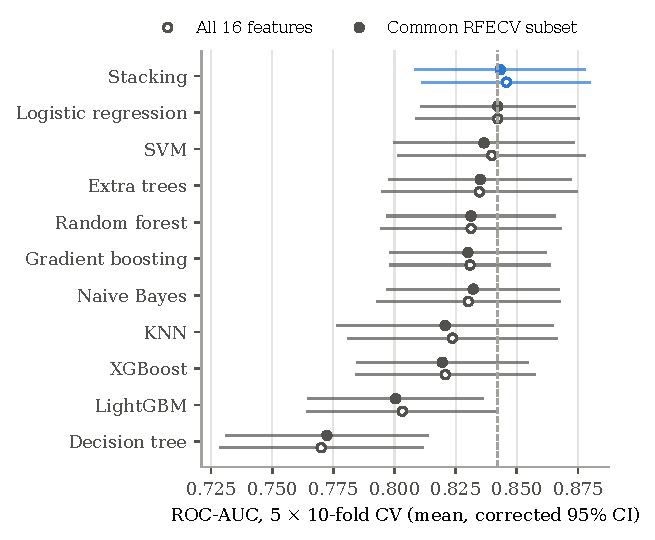
\includegraphics[width=0.75\linewidth]{fig2_cv_auc.pdf}
  \caption{Cross-validated ROC-AUC of each learner with all 16 features (open circles) and with the common RFECV subset (filled circles). Bars are Nadeau--Bengio corrected 95\% confidence intervals over 50 folds. The dashed line marks logistic regression on all features. The stacking ensemble is highlighted.}
  \label{fig:cv}
\end{figure}

\FloatBarrier
\subsection{Selected features and their stability}
Across the 50 outer folds, random-forest-ranked RFECV kept a median of 14 features (interquartile range 8--15; range 7--16). Seven features were kept in every fold: glucose, BMI and the engineered \texttt{Glucose\_BMI}, \texttt{Glucose\_Age}, \texttt{BMI\_Age}, \texttt{HOMA\_IR\_surrogate} and \texttt{Pedigree\_Age} (Fig.~\ref{fig:selection}). The diabetes pedigree function was kept in 94\% of folds. The thresholded flags were the weakest candidates: \texttt{Obese} was kept in 6\% of folds and \texttt{IGT\_2h} in 38\%. They largely duplicate information already carried by BMI and glucose.

Coefficient-ranked RFECV for logistic regression preferred a different, smaller subset (median 10.5 features; range 3--14). It kept glucose in every fold, and age, pregnancies and the pedigree function in more than 90\% of folds. It rarely kept blood pressure (2\%) and never kept skin-fold thickness. A core of glycaemic, adiposity and diabetes-pedigree predictors was therefore retained by both selectors, but the exact subset depended on the ranking criterion.

\begin{figure}[!htbp]
  \centering
  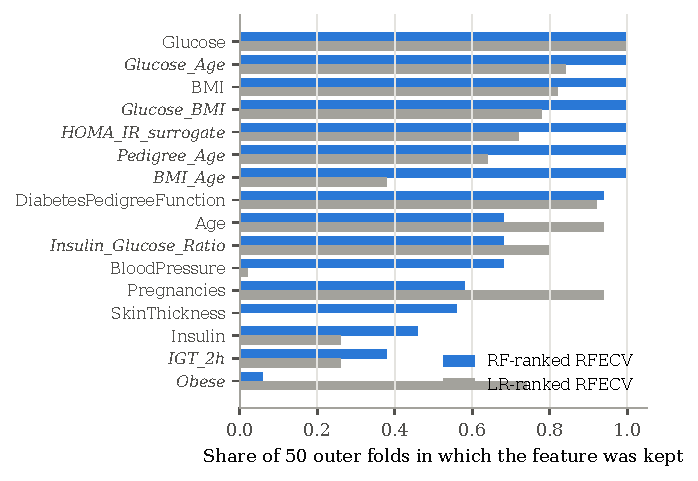
\includegraphics[width=0.75\linewidth]{fig3_selection.pdf}
  \caption{Proportion of the 50 outer cross-validation folds in which each candidate feature was retained by random-forest-ranked RFECV (the common protocol) and by coefficient-ranked RFECV for logistic regression. Engineered features are shown in italics.}
  \label{fig:selection}
\end{figure}

\FloatBarrier
\subsection{Internal hold-out performance}
On the 154 hold-out patients (Table~\ref{tab:holdout}, Fig.~\ref{fig:rocpr}), the stacking + RFECV pipeline reached a ROC-AUC of 0.822 (95\% CI 0.756--0.888), sensitivity 0.815 (0.709--0.915), specificity 0.740 (0.649--0.823), MCC 0.532 (0.403--0.658) and F1 0.710. It correctly identified 44 of 54 patients with diabetes. Among the evaluated configurations it had the highest observed sensitivity, F1 and MCC on this split. However, the confidence intervals of all models overlapped widely. No ROC-AUC difference between the stacking + RFECV pipeline and any comparator was statistically significant (DeLong test; differences from $-0.004$ to $+0.013$; smallest Holm-adjusted $p = 0.89$). Supplementary Table~S2 gives all hold-out metrics. Random forest + RFECV (0.826) and XGBoost + RFECV (0.824) had slightly higher hold-out ROC-AUC, and average precision ranged from 0.683 (logistic regression) to 0.711 (random forest + RFECV).

\begin{table*}[!htbp]
\centering
\caption{Hold-out performance ($n = 154$, 54 with diabetes) at a 0.5 threshold. 95\% confidence intervals are shown in grey beneath: DeLong for ROC-AUC, percentile bootstrap (2000 resamples) otherwise. AP, average precision. The last column gives the ROC-AUC difference of stacking + RFECV minus the comparator, with Holm-adjusted DeLong $p$-values.}
\label{tab:holdout}
\footnotesize
\setlength{\tabcolsep}{3.5pt}
\resizebox{\textwidth}{!}{%
\begin{tabular}{lccccccl}
\toprule
Model & ROC-AUC & Sensitivity & Specificity & MCC & F1 & AP & $\Delta$AUC (adj.\ $p$) \\
\midrule
Stacking + RFECV & 0.822 & 0.815 & 0.740 & 0.532 & 0.710 & 0.696 & -- \\
 & {\scriptsize\color{gray}(0.756--0.888)} & {\scriptsize\color{gray}(0.709--0.915)} & {\scriptsize\color{gray}(0.649--0.823)} & {\scriptsize\color{gray}(0.403--0.658)} & {\scriptsize\color{gray}(0.615--0.797)} &  &  \\[2pt]
Stacking & 0.819 & 0.796 & 0.720 & 0.494 & 0.688 & 0.702 & +0.003 (1.000) \\
 & {\scriptsize\color{gray}(0.752--0.885)} & {\scriptsize\color{gray}(0.688--0.904)} & {\scriptsize\color{gray}(0.631--0.804)} & {\scriptsize\color{gray}(0.362--0.625)} & {\scriptsize\color{gray}(0.592--0.778)} &  &  \\[2pt]
Logistic regression & 0.811 & 0.741 & 0.740 & 0.464 & 0.667 & 0.683 & +0.011 (1.000) \\
 & {\scriptsize\color{gray}(0.744--0.878)} & {\scriptsize\color{gray}(0.625--0.862)} & {\scriptsize\color{gray}(0.649--0.825)} & {\scriptsize\color{gray}(0.325--0.606)} & {\scriptsize\color{gray}(0.564--0.763)} &  &  \\[2pt]
LR + LR-ranked RFECV & 0.809 & 0.722 & 0.740 & 0.447 & 0.655 & 0.684 & +0.013 (0.892) \\
 & {\scriptsize\color{gray}(0.741--0.876)} & {\scriptsize\color{gray}(0.608--0.846)} & {\scriptsize\color{gray}(0.649--0.825)} & {\scriptsize\color{gray}(0.309--0.591)} & {\scriptsize\color{gray}(0.551--0.753)} &  &  \\[2pt]
Random forest + RFECV & 0.826 & 0.685 & 0.760 & 0.434 & 0.643 & 0.711 & -0.004 (1.000) \\
 & {\scriptsize\color{gray}(0.761--0.892)} & {\scriptsize\color{gray}(0.564--0.804)} & {\scriptsize\color{gray}(0.673--0.840)} & {\scriptsize\color{gray}(0.290--0.573)} & {\scriptsize\color{gray}(0.537--0.739)} &  &  \\[2pt]
XGBoost + RFECV & 0.824 & 0.648 & 0.820 & 0.470 & 0.654 & 0.697 & -0.003 (1.000) \\
 & {\scriptsize\color{gray}(0.758--0.891)} & {\scriptsize\color{gray}(0.523--0.776)} & {\scriptsize\color{gray}(0.743--0.888)} & {\scriptsize\color{gray}(0.321--0.605)} & {\scriptsize\color{gray}(0.543--0.752)} &  &  \\[2pt]
SVM & 0.810 & 0.537 & 0.830 & 0.383 & 0.580 & 0.684 & +0.012 (1.000) \\
 & {\scriptsize\color{gray}(0.740--0.880)} & {\scriptsize\color{gray}(0.407--0.672)} & {\scriptsize\color{gray}(0.755--0.896)} & {\scriptsize\color{gray}(0.226--0.534)} & {\scriptsize\color{gray}(0.457--0.692)} &  &  \\[2pt]
\bottomrule

\end{tabular}}
\end{table*}

\begin{figure*}[!htbp]
  \centering
  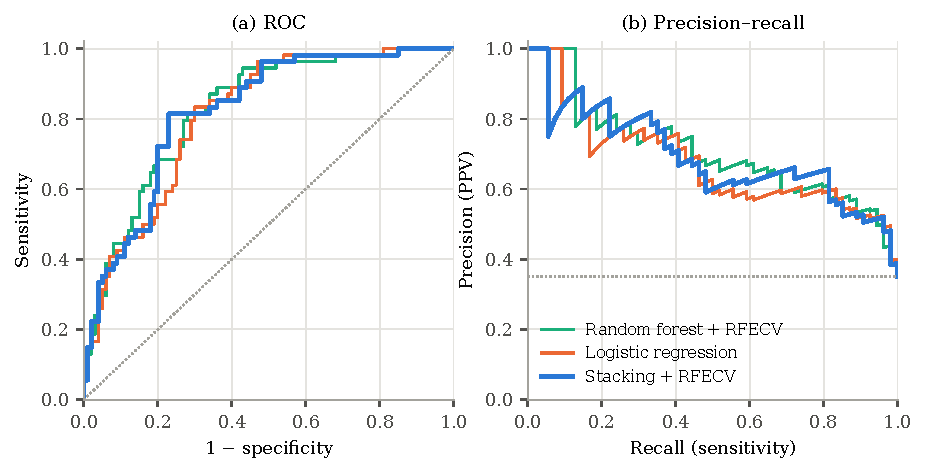
\includegraphics[width=0.9\textwidth]{fig4_roc_pr.pdf}
  \caption{Hold-out ROC (a) and precision--recall (b) curves for stacking + RFECV, logistic regression and random forest + RFECV. The dotted lines show chance performance and the outcome prevalence (0.35).}
  \label{fig:rocpr}
\end{figure*}

\FloatBarrier
\subsection{Calibration}
All class-weighted models overestimated risk (Table~\ref{tab:calibration}, Fig.~\ref{fig:calibration}). On the pooled development-set out-of-fold predictions, the calibration intercept was $-0.616$ for stacking + RFECV and $-0.623$ for logistic regression. This is almost exactly the logit of the outcome prevalence, $\operatorname{logit}(0.349) = -0.62$, which is consistent with the expected effect of balanced class weighting: weighting the classes equally corresponds to training at a prevalence of 50\%, which shifts the model intercept by about $-\operatorname{logit}(\pi)$ for prevalence $\pi$. We did not run a controlled experiment without class weights, so this explanation is supported by the arithmetic and by the well-calibrated unweighted Platt layer of the SVM, but it is not formally isolated. The calibration slope of the stack was close to one (1.002), so its spread of risks was appropriate and only its level was shifted. The Platt-calibrated SVM, whose probabilities are refitted without class weights, was well calibrated (intercept $-0.029$, slope 0.985) and had the lowest Brier score. On the hold-out set, the stack's intercept ($-0.624$) was unchanged and its slope fell to 0.866, compared with 0.756 for logistic regression.

\begin{table}[!htbp]
\centering
\caption{Calibration. Development values use pooled out-of-fold predictions ($614 \times 5$); hold-out Brier scores have bootstrap 95\% CIs. Ideal values: intercept 0, slope 1.}
\label{tab:calibration}
\footnotesize
\setlength{\tabcolsep}{3pt}
\begin{tabular}{lcccccc}
\toprule
& \multicolumn{3}{c}{Development (out-of-fold)} & \multicolumn{3}{c}{Hold-out} \\
\cmidrule(lr){2-4}\cmidrule(lr){5-7}
Model & Brier & Intercept & Slope & Brier (95\% CI) & Intercept & Slope \\
\midrule
Stacking + RFECV & 0.165 & -0.616 & 1.002 & 0.177 {\scriptsize\color{gray}(0.143--0.213)} & -0.624 & 0.866 \\
Logistic regression & 0.163 & -0.623 & 0.899 & 0.181 {\scriptsize\color{gray}(0.147--0.219)} & -0.629 & 0.756 \\
Random forest + RFECV & 0.164 & -0.406 & 0.823 & 0.166 {\scriptsize\color{gray}(0.134--0.201)} & -0.338 & 0.776 \\
SVM & 0.156 & -0.029 & 0.985 & 0.169 {\scriptsize\color{gray}(0.135--0.205)} & +0.004 & 0.844 \\
\bottomrule

\end{tabular}
\end{table}

\begin{figure*}[!htbp]
  \centering
  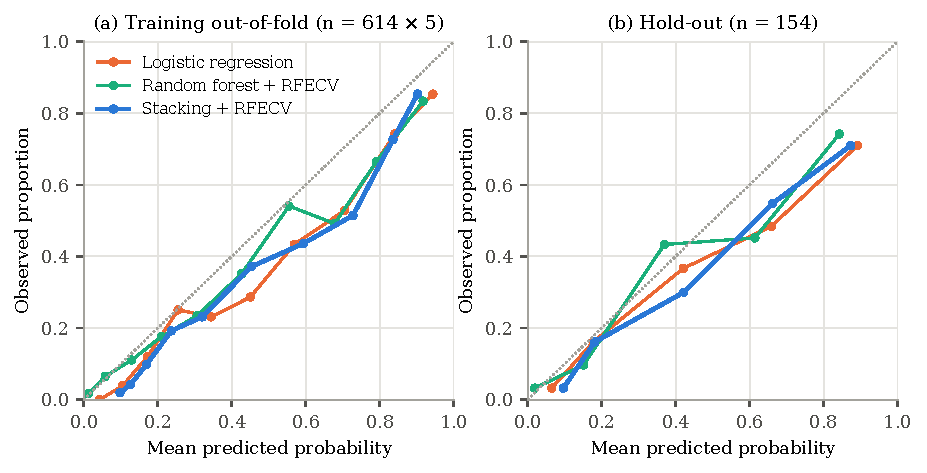
\includegraphics[width=0.9\textwidth]{fig5_calibration.pdf}
  \caption{Calibration curves (deciles of predicted risk) on (a) pooled development-set out-of-fold predictions and (b) the hold-out set (quintiles). Points below the diagonal indicate overestimated risk.}
  \label{fig:calibration}
\end{figure*}

\FloatBarrier
\subsection{Operating thresholds and decision-curve analysis}
Thresholds fixed on development-set out-of-fold predictions transferred reasonably to the hold-out set (Table~\ref{tab:thresholds}). For stacking + RFECV, the 80\%, 85\% and 90\% sensitivity targets gave hold-out sensitivities of 0.815, 0.852 and 0.907 and specificities of 0.66, 0.63 and 0.56, flagging 51\%--60\% of patients for confirmatory testing. The 95\% target gave a hold-out sensitivity of 0.926 (0.848--0.983), below target. With only 54 positive patients, each missed case changes sensitivity by 1.9 percentage points. Logistic regression gave very similar operating points; at the 95\% target it reached 0.963 with specificity 0.53. NPV was 0.87--0.96 across all thresholds and both models.

In this internal decision-curve analysis (Fig.~\ref{fig:dca}), all three models had higher net benefit than treating all or no patients across threshold probabilities from 0.10 to 0.55; logistic regression fell to zero net benefit at 0.60. The three curves were nearly identical up to a threshold of 0.45 (differences in net benefit of at most 0.03). Above 0.50, the stack retained slightly more net benefit than logistic regression, but this region is based on few patients.

\begin{table*}[!htbp]
\centering
\caption{Sensitivity-targeted operating points. Thresholds were chosen on development-set out-of-fold predictions and applied unchanged to the hold-out set. Bootstrap 95\% CIs are shown in grey beneath. ``Flagged'' is the proportion of hold-out patients referred for confirmatory testing.}
\label{tab:thresholds}
\footnotesize
\setlength{\tabcolsep}{4pt}
\resizebox{\textwidth}{!}{%
\begin{tabular}{lccccccc}
\toprule
Model & Target & Threshold & Sensitivity & Specificity & PPV & NPV & Flagged \\
\midrule
Stacking + RFECV & 80\% & 0.433 & 0.815 & 0.660 & 0.564 & 0.868 & 50.6\% \\
 &  &  & {\scriptsize\color{gray}(0.709--0.915)} & {\scriptsize\color{gray}(0.559--0.747)} & {\scriptsize\color{gray}(0.453--0.670)} & {\scriptsize\color{gray}(0.790--0.940)} &  \\[2pt]
Stacking + RFECV & 85\% & 0.348 & 0.852 & 0.630 & 0.554 & 0.887 & 53.9\% \\
 &  &  & {\scriptsize\color{gray}(0.754--0.942)} & {\scriptsize\color{gray}(0.529--0.723)} & {\scriptsize\color{gray}(0.442--0.658)} & {\scriptsize\color{gray}(0.809--0.957)} &  \\[2pt]
Stacking + RFECV & 90\% & 0.276 & 0.907 & 0.560 & 0.527 & 0.918 & 60.4\% \\
 &  &  & {\scriptsize\color{gray}(0.821--0.981)} & {\scriptsize\color{gray}(0.459--0.653)} & {\scriptsize\color{gray}(0.420--0.622)} & {\scriptsize\color{gray}(0.839--0.983)} &  \\[2pt]
Stacking + RFECV & 95\% & 0.212 & 0.926 & 0.520 & 0.510 & 0.929 & 63.6\% \\
 &  &  & {\scriptsize\color{gray}(0.848--0.983)} & {\scriptsize\color{gray}(0.423--0.621)} & {\scriptsize\color{gray}(0.408--0.606)} & {\scriptsize\color{gray}(0.855--0.984)} &  \\[2pt]
Logistic regression & 80\% & 0.413 & 0.852 & 0.650 & 0.568 & 0.890 & 52.6\% \\
 &  &  & {\scriptsize\color{gray}(0.754--0.942)} & {\scriptsize\color{gray}(0.551--0.738)} & {\scriptsize\color{gray}(0.458--0.671)} & {\scriptsize\color{gray}(0.814--0.958)} &  \\[2pt]
Logistic regression & 85\% & 0.345 & 0.852 & 0.620 & 0.548 & 0.886 & 54.5\% \\
 &  &  & {\scriptsize\color{gray}(0.754--0.942)} & {\scriptsize\color{gray}(0.520--0.710)} & {\scriptsize\color{gray}(0.438--0.654)} & {\scriptsize\color{gray}(0.806--0.956)} &  \\[2pt]
Logistic regression & 90\% & 0.284 & 0.889 & 0.580 & 0.533 & 0.906 & 58.4\% \\
 &  &  & {\scriptsize\color{gray}(0.804--0.968)} & {\scriptsize\color{gray}(0.480--0.674)} & {\scriptsize\color{gray}(0.427--0.633)} & {\scriptsize\color{gray}(0.829--0.970)} &  \\[2pt]
Logistic regression & 95\% & 0.212 & 0.963 & 0.530 & 0.525 & 0.964 & 64.3\% \\
 &  &  & {\scriptsize\color{gray}(0.903--1.000)} & {\scriptsize\color{gray}(0.431--0.630)} & {\scriptsize\color{gray}(0.419--0.624)} & {\scriptsize\color{gray}(0.903--1.000)} &  \\[2pt]
\bottomrule

\end{tabular}}
\end{table*}

\begin{figure}[!htbp]
  \centering
  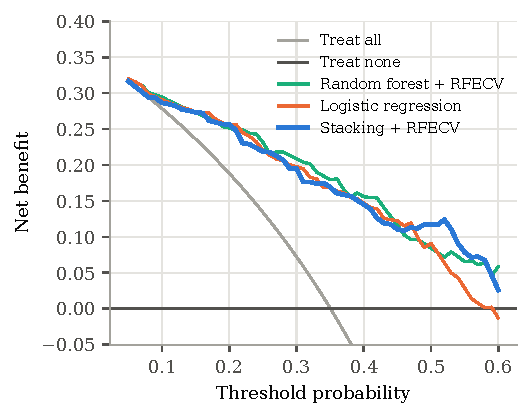
\includegraphics[width=0.6\linewidth]{fig6_dca.pdf}
  \caption{Decision curves on the hold-out set. Net benefit is shown against the threshold probability at which a patient would be referred for confirmatory testing.}
  \label{fig:dca}
\end{figure}

\FloatBarrier
\subsection{Sensitivity to missing-data handling}
The conclusions were robust to the imputation strategy (Table~\ref{tab:missing}). With iterative or $k$-NN imputation, ROC-AUC changed by at most $+0.005$ relative to median imputation for both logistic regression and RFECV + stacking (all $p \geq 0.45$). Adding missingness indicators did not help. It lowered the ROC-AUC of logistic regression slightly ($-0.010$, $p = 0.39$) and left RFECV + stacking unchanged ($-0.002$, $p = 0.50$), and RFECV retained on average only 1.2 of the five indicators. Under every strategy, stacking and logistic regression remained within 0.005 of each other.

\begin{table*}[!htbp]
\centering
\caption{Missing-data sensitivity analysis on the development set (10-fold cross-validation repeated twice; 20 folds). ROC-AUC values are means with corrected 95\% CIs. $\Delta$AUC is the paired difference from median imputation for the same model, with the corrected resampled $t$-test $p$-value.}
\label{tab:missing}
\resizebox{\textwidth}{!}{%
\begin{tabular}{llcccccl}
\toprule
Model & Imputation & Features & ROC-AUC (95\% CI) & MCC & Sens. & Brier & $\Delta$AUC ($p$) \\
\midrule
Logistic regression & Median & 16.0 & 0.846 (0.813--0.878) & 0.514 & 0.743 & 0.162 & reference \\
Logistic regression & Median + indicators & 21.0 & 0.836 (0.788--0.884) & 0.484 & 0.727 & 0.166 & -0.010 (0.387) \\
Logistic regression & Iterative (MICE-style) & 16.0 & 0.847 (0.814--0.879) & 0.517 & 0.753 & 0.162 & +0.001 (0.712) \\
Logistic regression & KNN ($k=10$) & 16.0 & 0.847 (0.813--0.880) & 0.505 & 0.743 & 0.162 & +0.001 (0.607) \\
\midrule
Stacking + RFECV & Median & 11.3 & 0.844 (0.804--0.883) & 0.498 & 0.752 & 0.164 & reference \\
Stacking + RFECV & Median + indicators & 13.3 & 0.841 (0.799--0.884) & 0.496 & 0.748 & 0.166 & -0.002 (0.503) \\
Stacking + RFECV & Iterative (MICE-style) & 14.0 & 0.848 (0.815--0.880) & 0.512 & 0.762 & 0.163 & +0.004 (0.594) \\
Stacking + RFECV & KNN ($k=10$) & 13.6 & 0.849 (0.814--0.884) & 0.501 & 0.759 & 0.163 & +0.005 (0.448) \\
\bottomrule

\end{tabular}}
\end{table*}


\FloatBarrier
\subsection{Explanation of predictions}
Glucose dominated the SHAP explanations of the stacking + RFECV pipeline (mean $|\mathrm{SHAP}| = 0.170$ on the probability scale), followed by BMI (0.074), age (0.055), the diabetes pedigree function (0.038) and pregnancies (0.028) (Fig.~\ref{fig:shap}). Insulin, skin-fold thickness and blood pressure contributed little (at most 0.015). Higher glucose, BMI, age and pedigree values consistently increased the predicted probability. These inputs contributed most to the model's predictions, in directions that agree with established risk factors; as model attributions, they do not measure causal effects. Because the outcome itself is largely defined by 2-h post-load glucose, the dominance of glucose in particular should not be interpreted as evidence of independent causal importance.

\begin{figure}[!htbp]
  \centering
  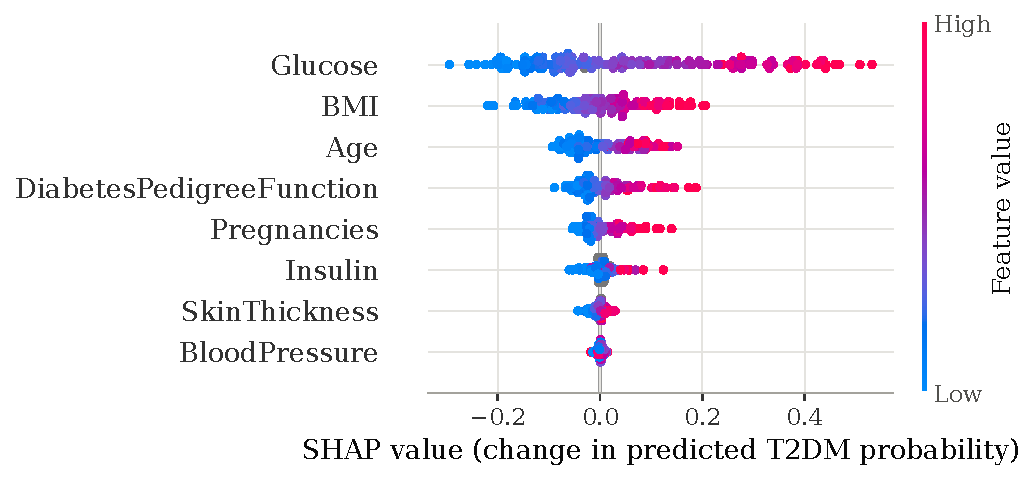
\includegraphics[width=0.8\linewidth]{fig7_shap.pdf}
  \caption{SHAP values of the hold-out predictions of the stacking + RFECV pipeline, expressed in the eight raw clinical inputs. Each point is one patient; colour shows the feature value.}
  \label{fig:shap}
\end{figure}

\section{Discussion}
\label{sec:discussion}

\subsection{Principal findings}
Under a validation design in which every data-dependent step was re-fitted inside each split, combining RFECV with an eight-learner stacking ensemble did not improve discrimination over regularised logistic regression on the PIMA cohort. Across 50 cross-validation folds, the stacks and logistic regression differed by less than 0.005 in ROC-AUC, and no difference approached significance after accounting for correlated folds and multiple comparisons. The same held on the hold-out set, where every DeLong comparison was non-significant. The higher hold-out sensitivity, F1 and MCC of RFECV + stacking (0.815, 0.710 and 0.532) are best read as the highest observed values on one 154-patient split, not as evidence of superiority. Its bootstrap confidence intervals overlap those of every comparator.

This null result is itself informative. It agrees with the systematic finding that flexible ML methods offer no average discrimination benefit over logistic regression in clinical prediction~\cite{christodoulou2019}. It also contrasts with the very high accuracies (0.90--0.98) sometimes reported for complex pipelines on the same 768 patients~\cite{zhou2023boruta,shams2025rfegru}. We cannot reproduce or audit those studies. However, a dataset with eight routine variables, a 35\% prevalence and a cross-validated ROC-AUC ceiling near 0.85 leaves little room for such gains. Validation design, especially preprocessing and feature selection outside the resampling loop~\cite{ambroise2002selection,kapoor2023leakage}, should be the first explanation considered for them.

\subsection{What RFECV and stacking contribute}
RFECV reduced the inputs by about a quarter with no loss of discrimination and identified a stable core of glycaemic, adiposity and family-history information, consistent with the SHAP analysis. The engineered interactions (\texttt{Glucose\_BMI}, \texttt{Glucose\_Age}, \texttt{BMI\_Age}, \texttt{HOMA\_IR\_surrogate}, \texttt{Pedigree\_Age}) were consistently preferred over thresholded flags and over raw blood pressure or skin-fold thickness. Two caveats apply. First, the selected size varied widely between folds (7--16 features) because the RFECV score curve is flat above about six features. A one-standard-error rule or stability selection~\cite{meinshausen2010stability} would yield smaller and more reproducible subsets. Second, the subset depended on the ranking estimator: coefficient-ranked RFECV for logistic regression chose different features than random-forest-ranked RFECV. The common protocol used here ensures a fair, identical selection procedure across learners, but it is not a learner-specific optimum, and results for individual learners should be read with that in mind.

Stacking added robustness rather than discrimination. It was never significantly worse than the best single learner, it did not require choosing a learner in advance, and at the default threshold it operated at higher sensitivity. Its meta-learner can also expose redundant base learners. Against these advantages stand higher computational cost (one RFECV + stacking fit took about 45~s, compared with milliseconds for logistic regression) and reduced transparency. On cohorts of this size, logistic regression remains a strong and simpler default.

\subsection{Calibration and thresholds matter more than the choice of learner}
The largest practical difference between configurations was not discrimination but calibration. Balanced class weights, which are widely used to raise sensitivity on imbalanced data, shifted predicted risks upwards by almost exactly the logit of the prevalence. The calibration slope stayed near one. The ranking of patients is therefore unaffected, but the predicted probabilities cannot be read as absolute risks without recalibration~\cite{vancalster2019calibration}. A simple intercept correction or Platt rescaling without class weights, fitted on out-of-fold predictions, would remove this offset. The well-calibrated SVM in our comparison shows the effect directly. Reporting only discrimination metrics, as most PIMA studies do, would have hidden this issue entirely.

Similarly, the default 0.5 threshold is arbitrary for screening. Thresholds chosen on development data for 80\%--90\% sensitivity transferred to the hold-out set within sampling error, at a cost of referring roughly half to 60\% of patients for confirmatory testing. Decision curves showed positive net benefit over the clinically plausible threshold range. However, all three models gave nearly identical net benefit, so the operating point matters more for clinical use than the choice between them.

\subsection{Missing data}
Almost half of the insulin values and 30\% of the skin-fold values were missing, so missingness itself might be expected to carry predictive information~\cite{sperrin2020missing}. In this cohort it did not. Missingness indicators slightly reduced discrimination, and iterative or $k$-NN imputation gave the same results as the simpler median imputation. The low SHAP contributions of insulin and skin-fold thickness agree with this. Whatever information these partially observed variables carry is largely redundant with glucose and BMI. Median imputation fitted within training folds was therefore adequate for this PIMA analysis under the evaluated alternatives; this may not hold in other cohorts, particularly where tests are ordered selectively.


\subsection{Limitations}
\begin{itemize}
  \item \textbf{One small, specific cohort.} PIMA comprises 768 women of one ethnic group from a single study. The results may not transfer to men, other populations or contemporary diagnostic criteria based on HbA1c. With 268 events and 16 candidate predictors, the cohort is also small for flexible model development~\cite{riley2020samplesize}.
  \item \textbf{No external validation.} Repeated cross-validation and a hold-out set estimate internal performance only. Validation on independent cohorts, such as population surveys with OGTT measurements, is needed before any clinical use.
  \item \textbf{One hold-out split.} With 54 positive hold-out patients, confidence intervals are wide. We therefore base inference on the 50-fold repeated cross-validation and treat hold-out results as confirmatory.
  \item \textbf{Fixed hyperparameters.} Learners were not tuned, to avoid an additional selection loop. Nested tuning could improve individual learners slightly, although the cross-validated ceiling suggests limited headroom.
  \item \textbf{Post-load measurements.} PIMA glucose and insulin are 2-h OGTT values, so \texttt{HOMA\_IR\_surrogate} is not a clinical HOMA-IR, and the model applies to settings where an OGTT has already been performed.
\end{itemize}

\subsection{Future work}
Future work should (i) validate the pipeline externally on larger, more diverse cohorts; (ii) incorporate recalibration and threshold selection into the nested pipeline; (iii) compare RFECV with stability selection and with learner-specific nested RFECV; and (iv) assess fairness and transportability across sex and ethnicity, as recommended by TRIPOD+AI~\cite{collins2024tripodai}.

\section{Conclusion}
\label{sec:conclusion}

We evaluated a leakage-controlled framework that combines RFECV with a heterogeneous stacking ensemble for T2DM prediction, using repeated cross-validation with corrected inference, an untouched hold-out set, calibration, threshold and decision-curve analysis, and SHAP explanations. RFECV produced compact feature sets built on glucose, BMI, family history and their interactions, without loss of discrimination. The stacking ensemble achieved the highest observed hold-out sensitivity (0.815), F1 (0.710) and MCC (0.532) on this split. However, across 50 cross-validation folds and on the hold-out set, it did not discriminate significantly better than regularised logistic regression (cross-validated ROC-AUC 0.843 versus 0.842). Class weighting produced a systematic overestimation of risk that discrimination metrics do not reveal. On small clinical tabular datasets, increased ensemble complexity therefore does not by itself improve prediction. The main value of such a framework lies in rigorous, leakage-free evaluation, sensitivity-oriented operating points and transparent reporting of calibration and clinical utility.

\section*{CRediT authorship contribution statement}
%% TODO(author): adjust if there are co-authors.
\textbf{Subrahmanyam Tanala:} Conceptualization, Methodology, Software, Formal analysis, Investigation, Visualization, Writing -- original draft, Writing -- review \& editing.

\section*{Declaration of competing interest}
The author declares no known competing financial interests or personal relationships that could have appeared to influence the work reported in this paper.

\section*{Funding}
This research did not receive any specific grant from funding agencies in the public, commercial, or not-for-profit sectors.

\section*{Ethics statement}
This study used only the publicly available, de-identified PIMA Indians Diabetes dataset. No new data were collected from human participants, so ethical approval and informed consent were not required.

\section*{Data and code availability}
The PIMA Indians Diabetes dataset is publicly available~\cite{pimadata} and is included in the repository as \texttt{data/diabetes.csv} (768 records, header row added). All code, configuration files, fold-level results and the scripts that regenerate every table and figure in this article are available at \url{https://github.com/subrahmanyamtanala-rgb/T2D}. %% TODO(author): make the repository public, or provide an anonymised review link, and add a release DOI (e.g. Zenodo) before submission.
All reported numbers were produced from commit \texttt{e23102d}. The full analysis can be reproduced with \texttt{python -m t2d.analysis --stage cv}, \texttt{--stage holdout} and \texttt{--stage missing}, followed by \texttt{python paper/make\_assets.py}.

\section*{Supplementary material}
Supplementary material includes the nested validation diagram (Fig.~S1), the full statistical testing procedure, results for all configurations and metrics (Tables S1--S3), a TRIPOD+AI reporting map (Table S4), the list of all 23 configurations (Table S5), and reproduction instructions including every random seed.

\section*{Declaration of generative AI and AI-assisted technologies in the manuscript preparation process}
%% TODO(author): Elsevier requires this disclosure; edit it to describe your actual use.
During the preparation of this work the author used Claude (Anthropic) to assist with software development, statistical analysis code and drafting of the manuscript text. After using this tool, the author reviewed and edited the content as needed and takes full responsibility for the content of the published article.


\bibliographystyle{elsarticle-num}
\bibliography{references}

\end{document}
